\documentclass[11pt]{article}

%imports
\usepackage[utf8]{inputenc}
\usepackage[T1]{fontenc}
\usepackage{amsmath}
\usepackage{amsfonts}
\usepackage{amssymb}
\usepackage{footnote}
\usepackage{url}
\usepackage{natbib}

%images and image path
\usepackage{graphicx}
\usepackage{subfig}
\graphicspath{ {./images/} }

%custom commands
\newcommand{\N}{\mathcal{N}}
\newcommand{\num}{\text{num}}
\newcommand{\obs}{\text{obs}}
\newcommand{\D}{\mathfrak{D}}
\newcommand{\Ro}{\mathcal{R}_0}
\newcommand{\lap}{{\mathcal{L}}}
\renewcommand\vec{\mathbf}
\newcommand{\mat}[1]{\mathsf{#1}}

%insitute command
\usepackage{etoolbox}
\makeatletter
\providecommand{\institute}[1]{% add institute to \maketitle
	\apptocmd{\@author}{\end{tabular}
	\par
	\begin{tabular}[t]{c}
		\small \textit{#1}}{}{}
}
\makeatother

%margins
\usepackage[letterpaper, total={6.5in, 9.5in}]{geometry}

%opening
\title{Reaction-diffusion spatial modeling of COVID-19 in Chicago}
\author{Trent Gerew\thanks{\texttt{tgerew@hawk.iit.edu}}}
\institute{Department of Applied Mathematics, Illinois Institute of Technology, Chicago, Illinois}

\begin{document}

\maketitle

\section{Model Setup}

	\begin{figure}[h!]
		\centering
		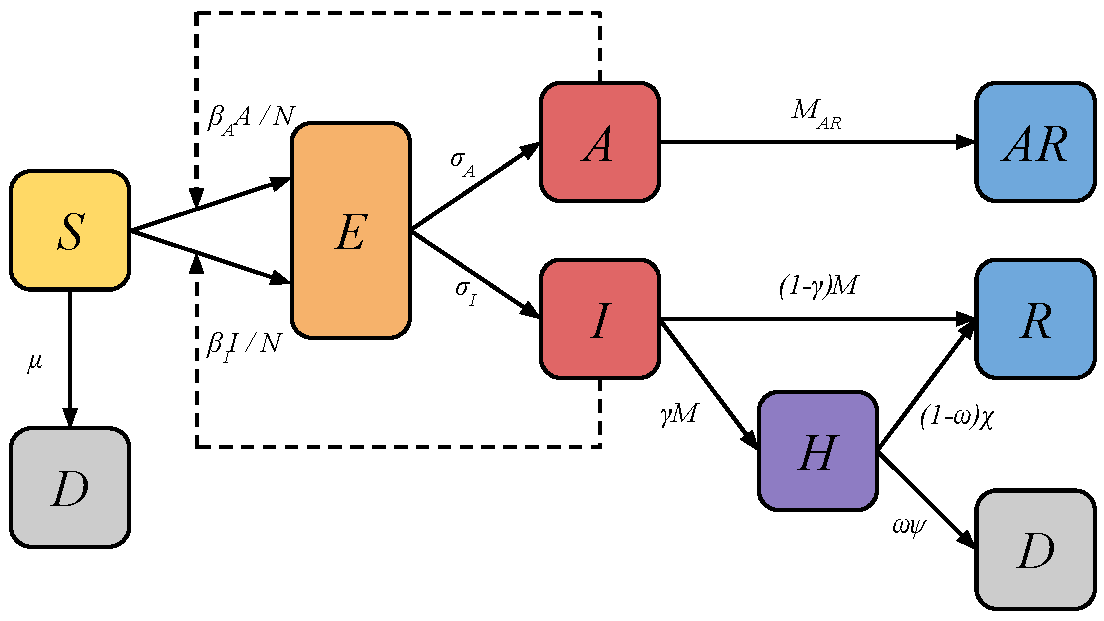
\includegraphics[height=6cm]{full-model}
		\label{fig:model}
		\caption{Schematic diagram of the model. The dashed lines indicate the interaction of the infected populations with the susceptible populations that leads to infection.}
	\end{figure}

	\begin{align}
		S_t &=	\D_S \Delta S - \beta_{SA} S A - \beta_{SI} S I - \mu S, \\
		E_t	&=	\D_E \Delta E + \beta_{SA} S A + \beta_{SI} S I - (\sigma_A + \sigma_I) E, \\
		A_t	&=	\D_A \Delta A + \sigma_A E - M_{AR} A, \\
		I_t	&=	\sigma_I E - M I, \\
		H_t	&=	\gamma M I - (1 - \omega) \chi H - \omega \chi H, \\
		R_t	&=	(1 - \gamma) M I + (1 - \omega) \chi H, \\
		D_t	&=	\omega \chi H.
	\end{align}
	
	\begin{table}[h]
		\centering
		\caption{Population values for Chicago.}
		\label{tab:populations}
		\begin{tabular}{ c c c }
			\hline
			\hline
			&	&	Population \\
			\hline
			Total population		&	$N$		&	2,695,598 \\
			Initial infected		&	$I_0$	&	127	\\
			Initial hospitalized	&	$H_0$	&	30 \\
			Initial deceased		&	$D_0$	&	6 \\
			\hline
			\hline
		\end{tabular}
	\end{table}
	
	\begin{table}[h]
		\centering
		\caption{Parameters for Chicago: optimal (best-fitting), median and interquartile range, and variation range used in the optimization algorithm. Initial parameter guesses were uniformly sampled within these ranges.}
		\label{tab:parameters}
		\begin{tabular}{ c c c c }
			\hline
			\hline
			&	&	Median (interquartile range)	&	Initial value \\
			\hline
			Population	&	$N$	&	2,695,598	& \\
			Initial population	&	$(I_0, R_0)$	&	(127, 2)	& \\
			Transmission rate, $S \rightarrow I$ [per day]	&	$\beta$\footnote{The transmission rate $\beta$ must be divided by $N$ when used in the ODE model.}	&	0.38206(0.38204-0.38209)	&	$c \in U[0,1]$ \\
			Transition rate, $I \rightarrow R$ [per day]	&	$\gamma$	&	 0.39656(0.39654-0.39659)	&	$c \in U[0.25,0.75]$ \\
			Diffusivity, $S$ [km$^2$/day]	&	$\D_S$	&	10	&	\\
			Diffusivity, $I$ [km$^2$/day]	&	$\D_I$	&	100	&	\\
			\hline
			\hline
		\end{tabular}
	\end{table}

\section{ODE Dynamics}
	We want to understand the trajectories of the dynamics of the ODE system under different initial conditions.
	To do this we first find the equilibrium points by solving
	$$S_t = E_t = A_t = I_t = H_t = R_t = D_t = 0$$
	simultaneously for $\vec{x} = (S, E, A, AR, I, H, R, D)$.
	The solutions of this system are of the form $\vec{x^*} = (0, 0 , 0, AR, 0, 0, R, D)$.
	This implies there are infinitely many non-isolated equilibrium points.
	We determine the stability of these equilibrium points by analyzing the linearized system near the points.
	The Jacobian of the system is
	\begin{equation}
		\mat{J} = \begin{pmatrix}
			- A \beta_{SA} - I \beta_{SI} - \mu	&	0						&	- S \beta_{SA}	&	0	&	- S \beta_{SI}	&	0									&	0	&	0	\\
			A \beta_{SA} + I \beta_{SI}			&	- \sigma_A - \sigma_I	&	S \beta_{SA}	&	0	&	S \beta_{SI}	&	0									&	0	&	0	\\
			0									&	\sigma_A				&	- M_{AR}		&	0	&	0				&	0									&	0	&	0	\\
			0									&	0						&	M_{AR}			&	0	&	0				&	0									&	0	&	0	\\
			0									&	\sigma_I				&	0				&	0	&	- M				&	0									&	0	&	0	\\
			0									&	0						&	0				&	0	&	M \gamma		&	- \chi (1 - \omega) - \psi \omega	&	0	&	0	\\
			0									&	0						&	0				&	0	&	M (1 - \gamma)	&	\chi (1 - \omega)					&	0	&	0	\\
			0									&	0						&	0				&	0	&	0				&	\psi \omega							&	0	&	0
		\end{pmatrix}
	\end{equation}
	Now evaluating $\mat{J}$ at the equilibrium point $\vec{x^*}$ and calculating the eigenvalues, we have
	\begin{equation}
		\vec{\lambda} = \{0 , 0, 0, - M, - M_{AR}, - \mu, - \sigma_A - \sigma_I, - \chi + \chi \omega - \psi \omega \}.
	\end{equation}
	Note that the first three eigenvalues are 0, which implies the equilibrium points are non-isolated.
	This agrees with our earlier observation.
	
	The equilibrium points are stable when $\lambda_i < 0$ for $4 \leq i \leq 8$.
	Since all the system parameters are positive, this implies $\lambda_i < 0$ for $4 \leq i \leq 7$.
	Thus the stability depends on the sign of $\lambda_8$.
	There are two cases when $\lambda_8 = - \chi + \chi \omega - \psi \omega < 0$ is true:
	\begin{enumerate}
		\item $0 < \omega \leq 1$ implies $\lambda_8 < 0$, and
		\item $\omega > 1$ and $\chi < \frac{\psi \omega}{\omega - 1}$ implies $\lambda_8 < 0$.
	\end{enumerate}
	That is, whenever we have either of these conditions the equilibrium points are stable.
	We call this situation \textit{endemic}.
	If $\lambda_8 > 0$, the equilibrium points are unstable and the situation is an \textit{epidemic}.

\bibliographystyle{abbrv}
\bibliography{chicago-spatial-covid-draft}

\end{document}
